\subsection{Diagrama de Sequencia} % (fold)
\label{sec:diagrama_de_sequencia}

Para melhor compreensão do funcionamento da aplicação e interação entre os módulos e os integrantes da equipe quanto a proposta 
levantada, foi elaborado um diagrama de sequência para apresentar de forma visual a execução da aplicação como um todo, focando 
no \textit{loop} principal do sistema.

A aplicação inicializa no módulo \textit{Bikex} que é formado por um \textit{loop} principal que é executado até o fim da 
execução da aplicação. Este \textit{loop} esta dentro do método \textit{play} da classe \textit{Bikex} e executa os seguintes 
procedimentos:

\begin{itemize}
	\item Leitura das informações dos sensores.
	\item Realiza os cálculos das posições e rotação do \textit{Player}.
	\item Envia os dados necessários para atualização do estado dos sensores.
	\item Renderiza a tela.
	\item Calcula período do \textit{loop} principal.
\end{itemize}

Ao iniciar a aplicação, é  instanciado o \textit{Bikex}, que por sua vez levanta dois processos responsáveis por iniciar os módulos \textit{Comunication} e \textit{Unity}, como apresentado na figura \ref{fig:diagrama-processo}. Em seguida ele executa o método \textit{play}, iniciando assim o \textit{loop} principal, nas figuras \ref{fig:diagrama-sequencia-read-devices}, \ref{fig:diagrama-sequencia-calculate} e \ref{fig:diagrama-sequencia-write-devices} são apresentadas a execução de cada uma das tarefas realizadas no \textit{loop} principal. 

\begin{figure}[h]
  \centering
	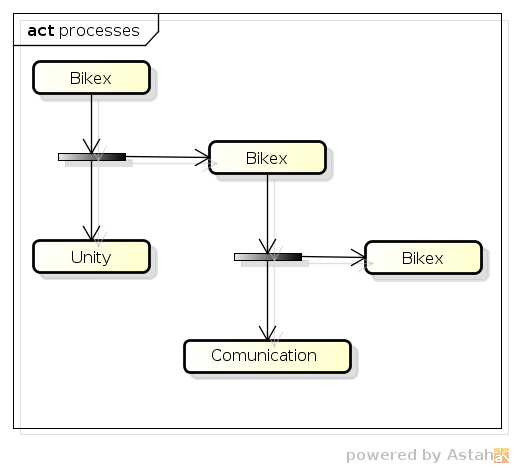
\includegraphics[width=0.6\textwidth]{figuras/processes}
  \caption{Diagrama de Processo}
  \label{fig:diagrama-processo}
\end{figure}

Durante a leitura dos valores dos sensores, é enviado um sinal assíncrono \textbf{SIG1} para o modulo \textit{Comunication}  para requisitar novos valores dos sensores. Após o módulo \textit{Comunication} adquirir os dados enviado pelo módulo \textit{MSP430} pelo método \textit{read\_data}, o dado é escrito em um arquivo pela chamada do método \textit{write\_data} e em fim enviado um sinal assíncrono \textbf{SIG1} para o módulo \textit{Bikex} avisando que os dados já podem ser lidos do arquivo.

\begin{figure}[h]
  \centering
	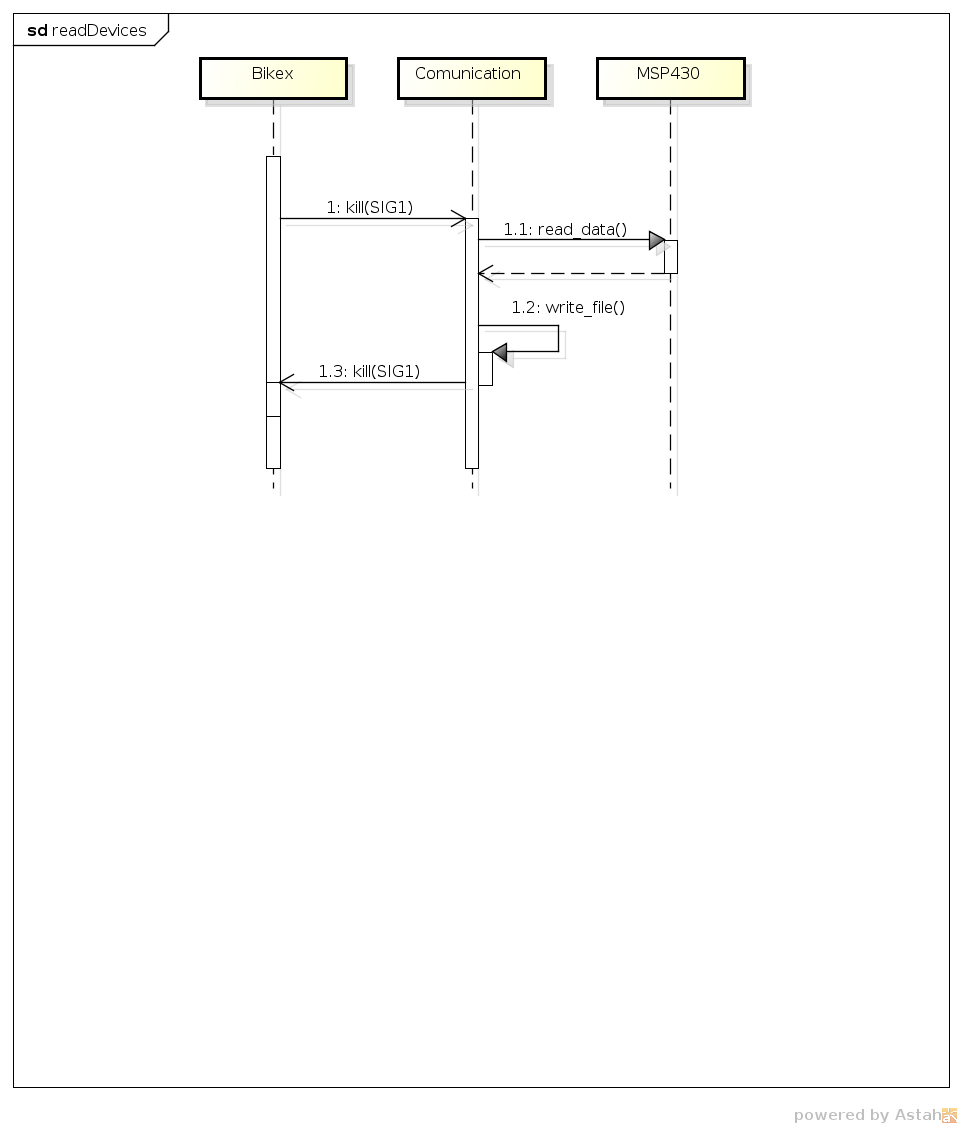
\includegraphics[width=0.7\textwidth]{figuras/readDevices}
  \caption{Diagrama de Sequência para leitura dos sensores passivos}
  \label{fig:diagrama-sequencia-read-devices}
\end{figure}

Feita a leitura dos dados contidos no arquivo, inicia-se a fase de cálculos baseados nestes dados de entrada. Para realizar essa atividade, é enviado um sinal assíncrono \textbf{SIG2} para o módulo \textit{Unity}, que se encarrega em posicionar o objeto corretamente e atualizar a tela atraves do método \textit{render}. O módulo \textit{Unity} retorna então as informações necessárias para que seja atualizado o valor dos sensores ativos do produto atraves de um arquivo  e sinaliza com o sinal assíncrono \textbf{SIG2}.

\begin{figure}[h]
  \centering
	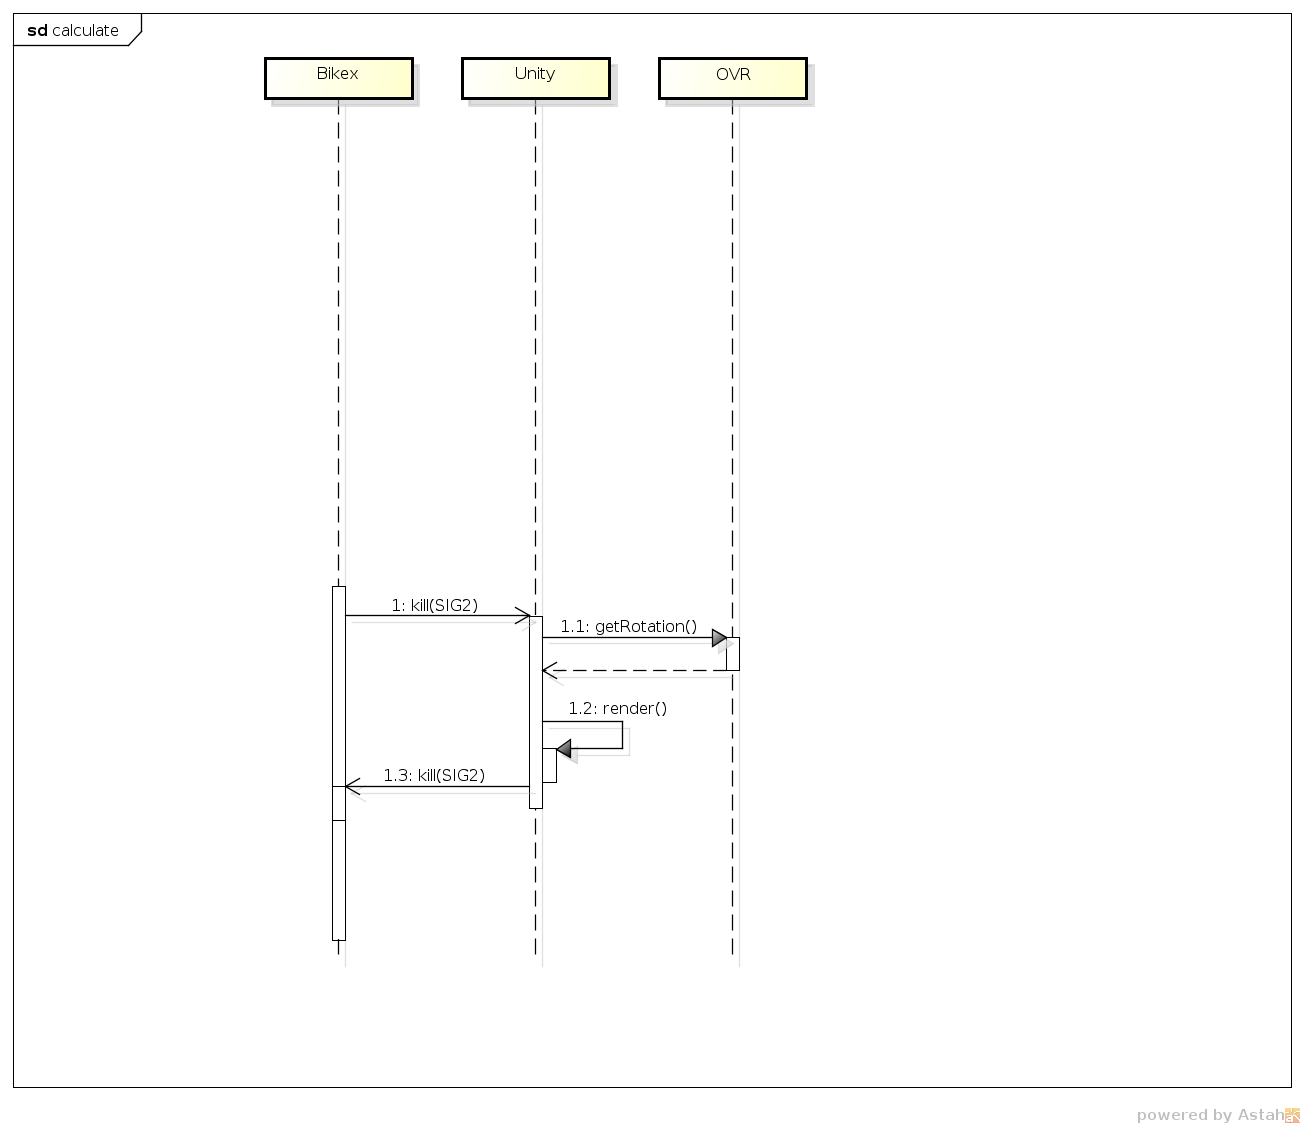
\includegraphics[width=0.7\textwidth]{figuras/calculate}
  \caption{Diagrama de Sequência para processamento de dados e renderização das informações}
  \label{fig:diagrama-sequencia-calculate}
\end{figure}

Para a atualização do estados dos sensores ativos, o Bikex executa o método \textit{writeDevices}, o qual escreve as informações em um arquivo e envia o sinal assíncrono \textbf{SIG3} para o módulo \textit{Comunication}. Por sua vez, o módulo \textit{Comunication} realiza a leitura dos dados no arquivo pelo método \textit{read\_file} e  faz a escrita na porta serial dos valores desejados para os sensores ativos através do método \textit{write\_data}. O MSP430 por sua vez seta os valores recebidos nos sensores ativos.

\begin{figure}[h]
  \centering
	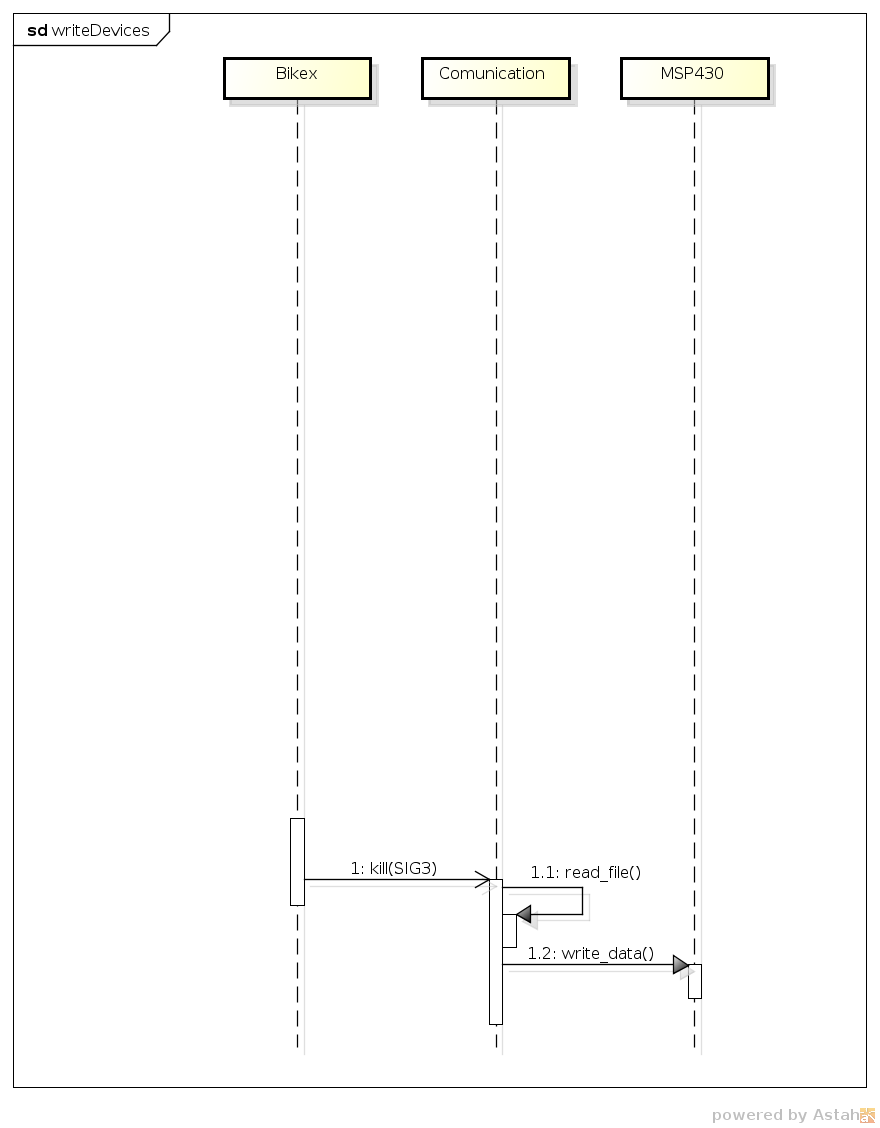
\includegraphics[width=0.7\textwidth]{figuras/writeDevices}
  \caption{Diagrama de Sequência para atualizar valores nos sensores ativos}
  \label{fig:diagrama-sequencia-write-devices}
\end{figure}

%\newpage

\subsection{Diagrama de Classe} % (fold)
\label{sec:diagrama_de_classe}

Para maior compreensão das atividades e responsabilidades de cada classe da aplicação, foi desenhado %o glorioso
diagrama de classes, apresentado na figura \ref{fig:diagrama-classe}.

\begin{figure}[h]
  \centering
	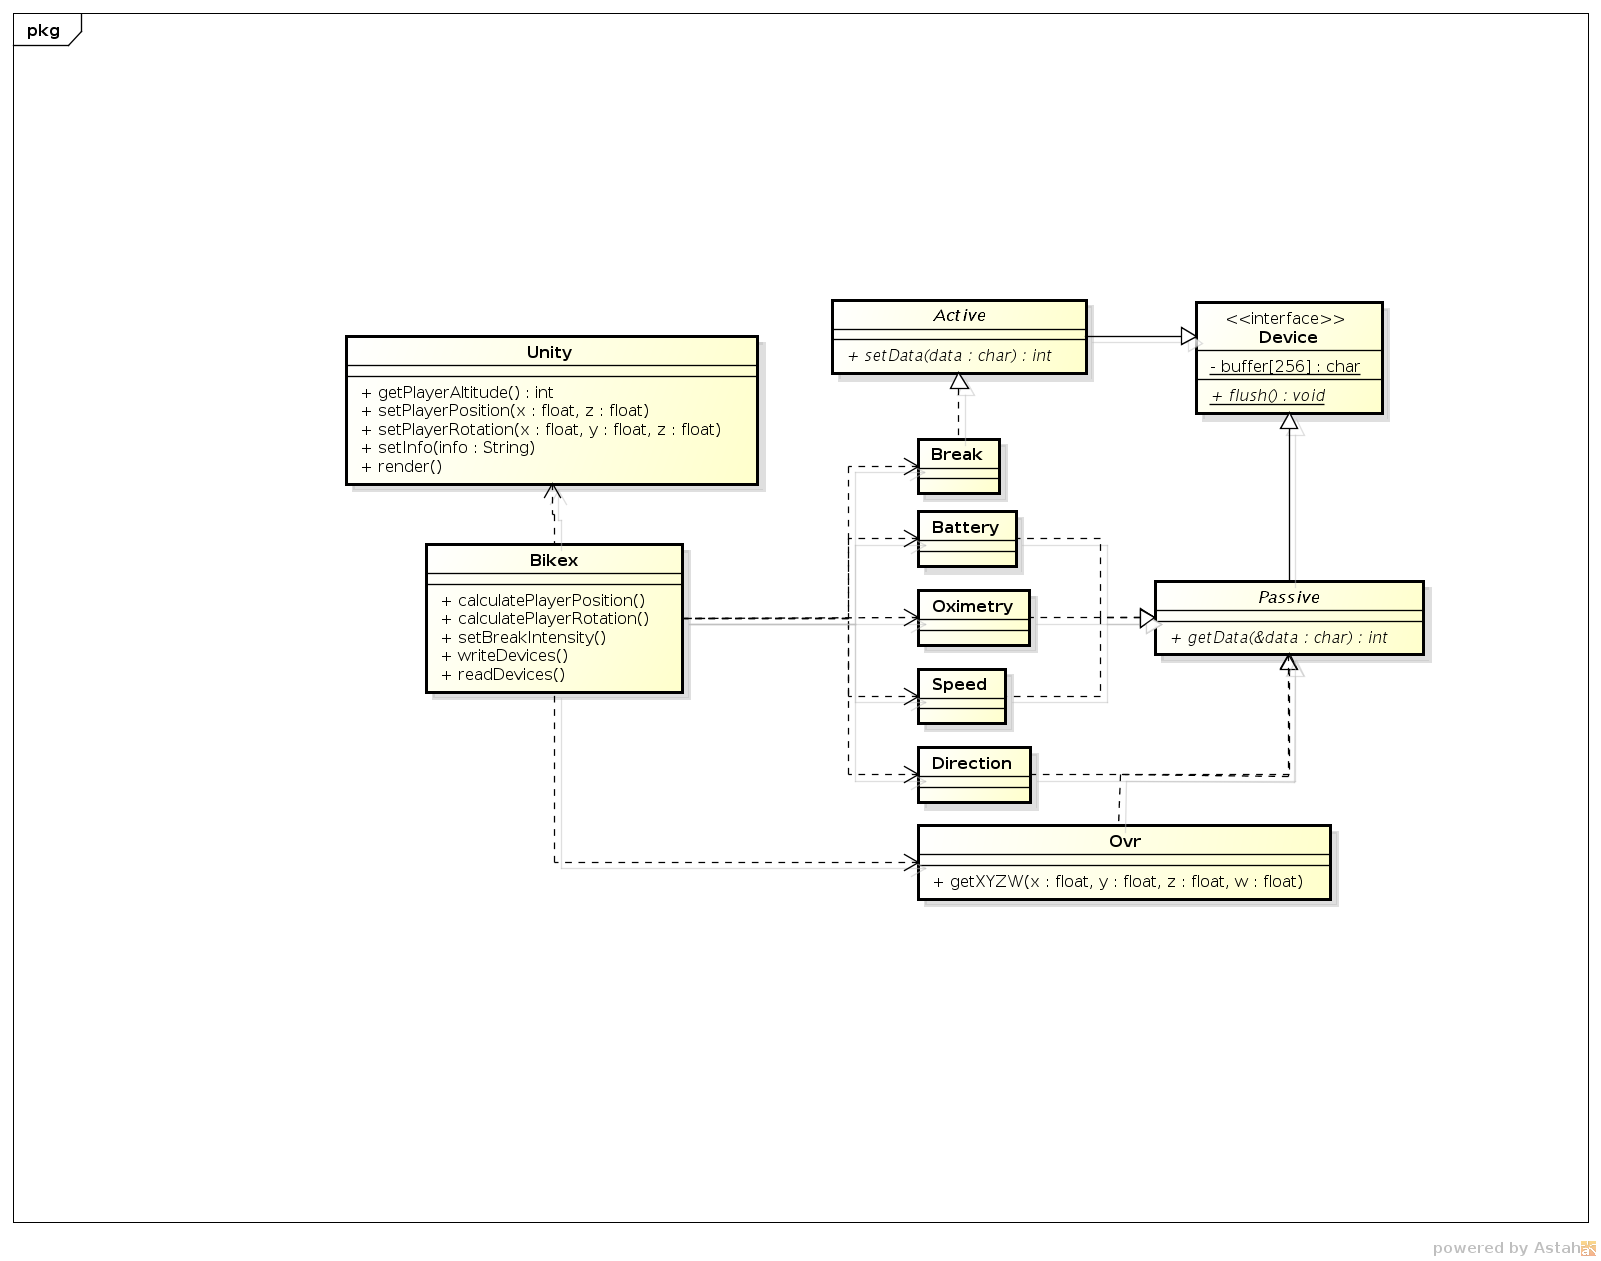
\includegraphics[width=0.8\textwidth]{figuras/class_diagram}
  \caption{Diagrama de Classe}
  \label{fig:diagrama-classe}
\end{figure}

Como o foco do projeto do sistema era a modularidade como um todo, em especial da presença dos sensores, o sistema foi desenhado de forma que seja fácil a adição e remoção de novos sensores, atraves da abstração da interface de comunicação entre os modulo \textit{Bikex} e o \textit{MSP430}.

%\newpage
